\usepackage{tikz}
\usetikzlibrary{positioning,shapes,shadows,arrows,fit}

\tikzstyle{struct}=[rectangle, draw=black, text centered, anchor=north, text=black, text width=4cm]
\tikzstyle{thread}=[rectangle, draw=black, text centered, anchor=north, text=black, text width=4cm]
\tikzstyle{app}=[rectangle, draw=black, text centered, anchor=north, text=black, text width=3cm]

\tikzstyle{title}=[font=\fontsize{6}{6}\color{black!50}]

\usetikzlibrary{arrows.meta}
\tikzset{>={Latex[scale=1.2]}} 


\newcommand{\architecture}{
\begin{figure}[h!]
\centering
    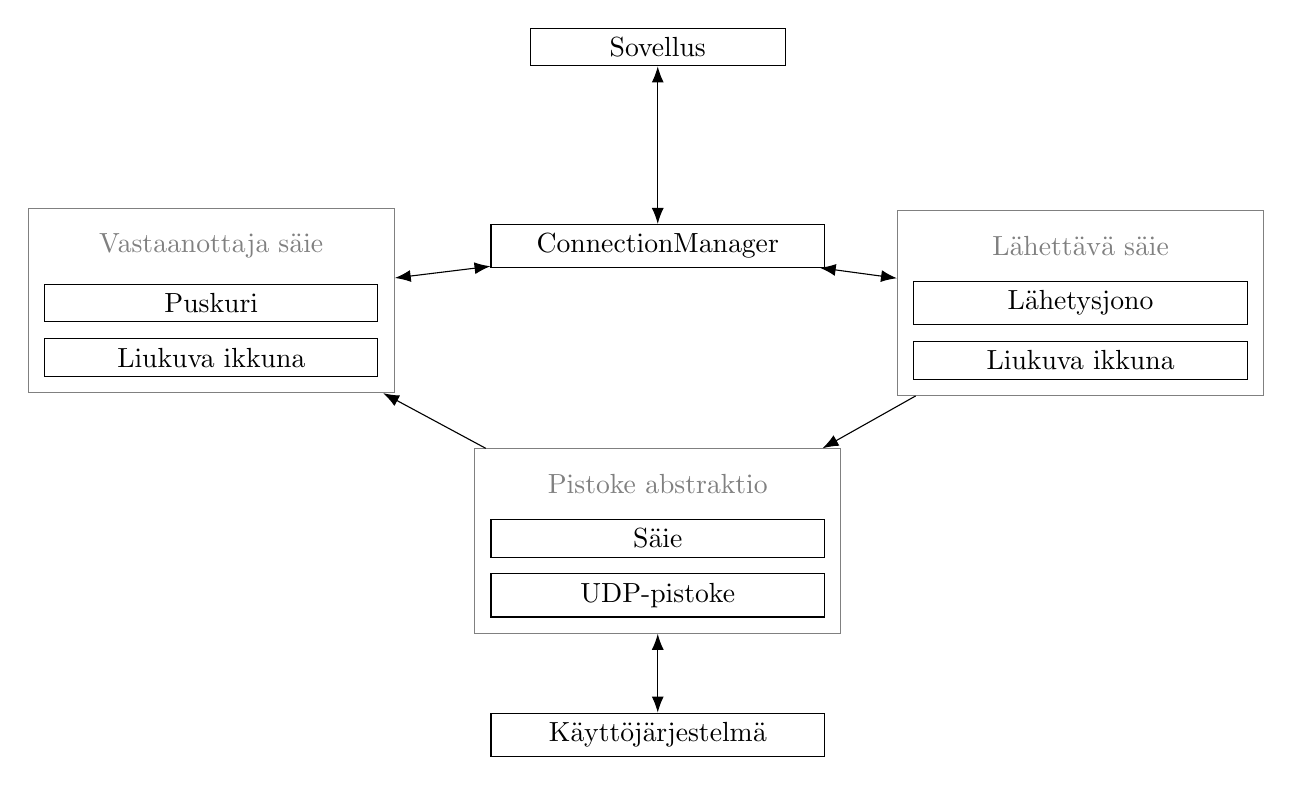
\begin{tikzpicture}[node distance=2cm]
        \node(app)[app]{
            Sovellus
        };
        \node(ConnectionManager)[struct, below=of app] {
            ConnectionManager
        };
        \draw[<->] (app) -- (ConnectionManager);

        
       \node(rthread)[title, left=of ConnectionManager]{
            Vastaanottaja säie
       };
       
        
       \node(buffer)[struct, below=0.2cm of rthread] {
            Puskuri 
       };
       \node(rwindow)[struct, below=0.2cm of buffer] {
            Liukuva ikkuna 
       };

        \node (rthread_box) [inner sep=0.2cm, draw=black!50, fit={(rthread) (buffer) (rwindow)}] {};

        \draw[<->] (rthread_box) -- (ConnectionManager);
       
       \node(tthread)[title, right=of ConnectionManager]{
            Lähettävä säie
       };
       
        
       \node(queue)[struct, below=0.2cm of tthread] {
            Lähetysjono
       };
       
       \node(twindow)[struct, below=0.2cm of queue] {
            Liukuva ikkuna 
       };
       
        \node (tthread_box) [inner sep=0.2cm, draw=black!50, fit={(tthread) (queue) (twindow)}] {};
        
        \draw[<->] (tthread_box) -- (ConnectionManager);


       \node(socket)[title, below=of ConnectionManager, yshift=-0.5cm]{
            Pistoke abstraktio
       };
       
       \node(socketthread)[struct, below=0.2cm of socket]{
            Säie
       };
       
       \node(udp_socket)[struct, below=0.2cm of socketthread]{
            UDP-pistoke
       };
       
        \node (socket_box) [inner sep=0.2cm, draw=black!50, fit={(socket) (socketthread) (udp_socket) }] {};
       
       \node(os)[struct, below=1cm of socket_box]{
            Käyttöjärjestelmä
       };
       
        \draw[<->] (socket_box) -- (os);
        
        \draw[->] (tthread_box) -- (socket_box);
        \draw[->] (socket_box) -- (rthread_box);
    \end{tikzpicture}
    \caption{Arkkitehtuuridiagrammi} \label{fig:arkkitehtuuri}
\end{figure}
}